The primary objective of this thesis is to assess the potentials and limitations of a self developed APR pipeline prototype. We aim to answer the following research questions to evaluate the system's capabilities and impact on the software development process:

\begin{itemize}
    \item \textbf{RQ1:} How can LLM-based automated bug fixing be effectively and efficiently integrated into a CI pipeline?
    \item \textbf{RQ2:} What are the key potentials of this integrated approach in terms of repair success rate, cost-effectiveness and developer workflow enhancement?
    \item \textbf{RQ3:} What are the primary limitations and challenges, such as performance overhead, accuracy, and security, of using LLM-based APR within a CI context?
\end{itemize}

For answering these questions we streamlined this process into three phases Preparation, Implementation and Evaluation, shown in Figure \ref{fig:method-overview}.

\begin{figure}[H]
    \centering
    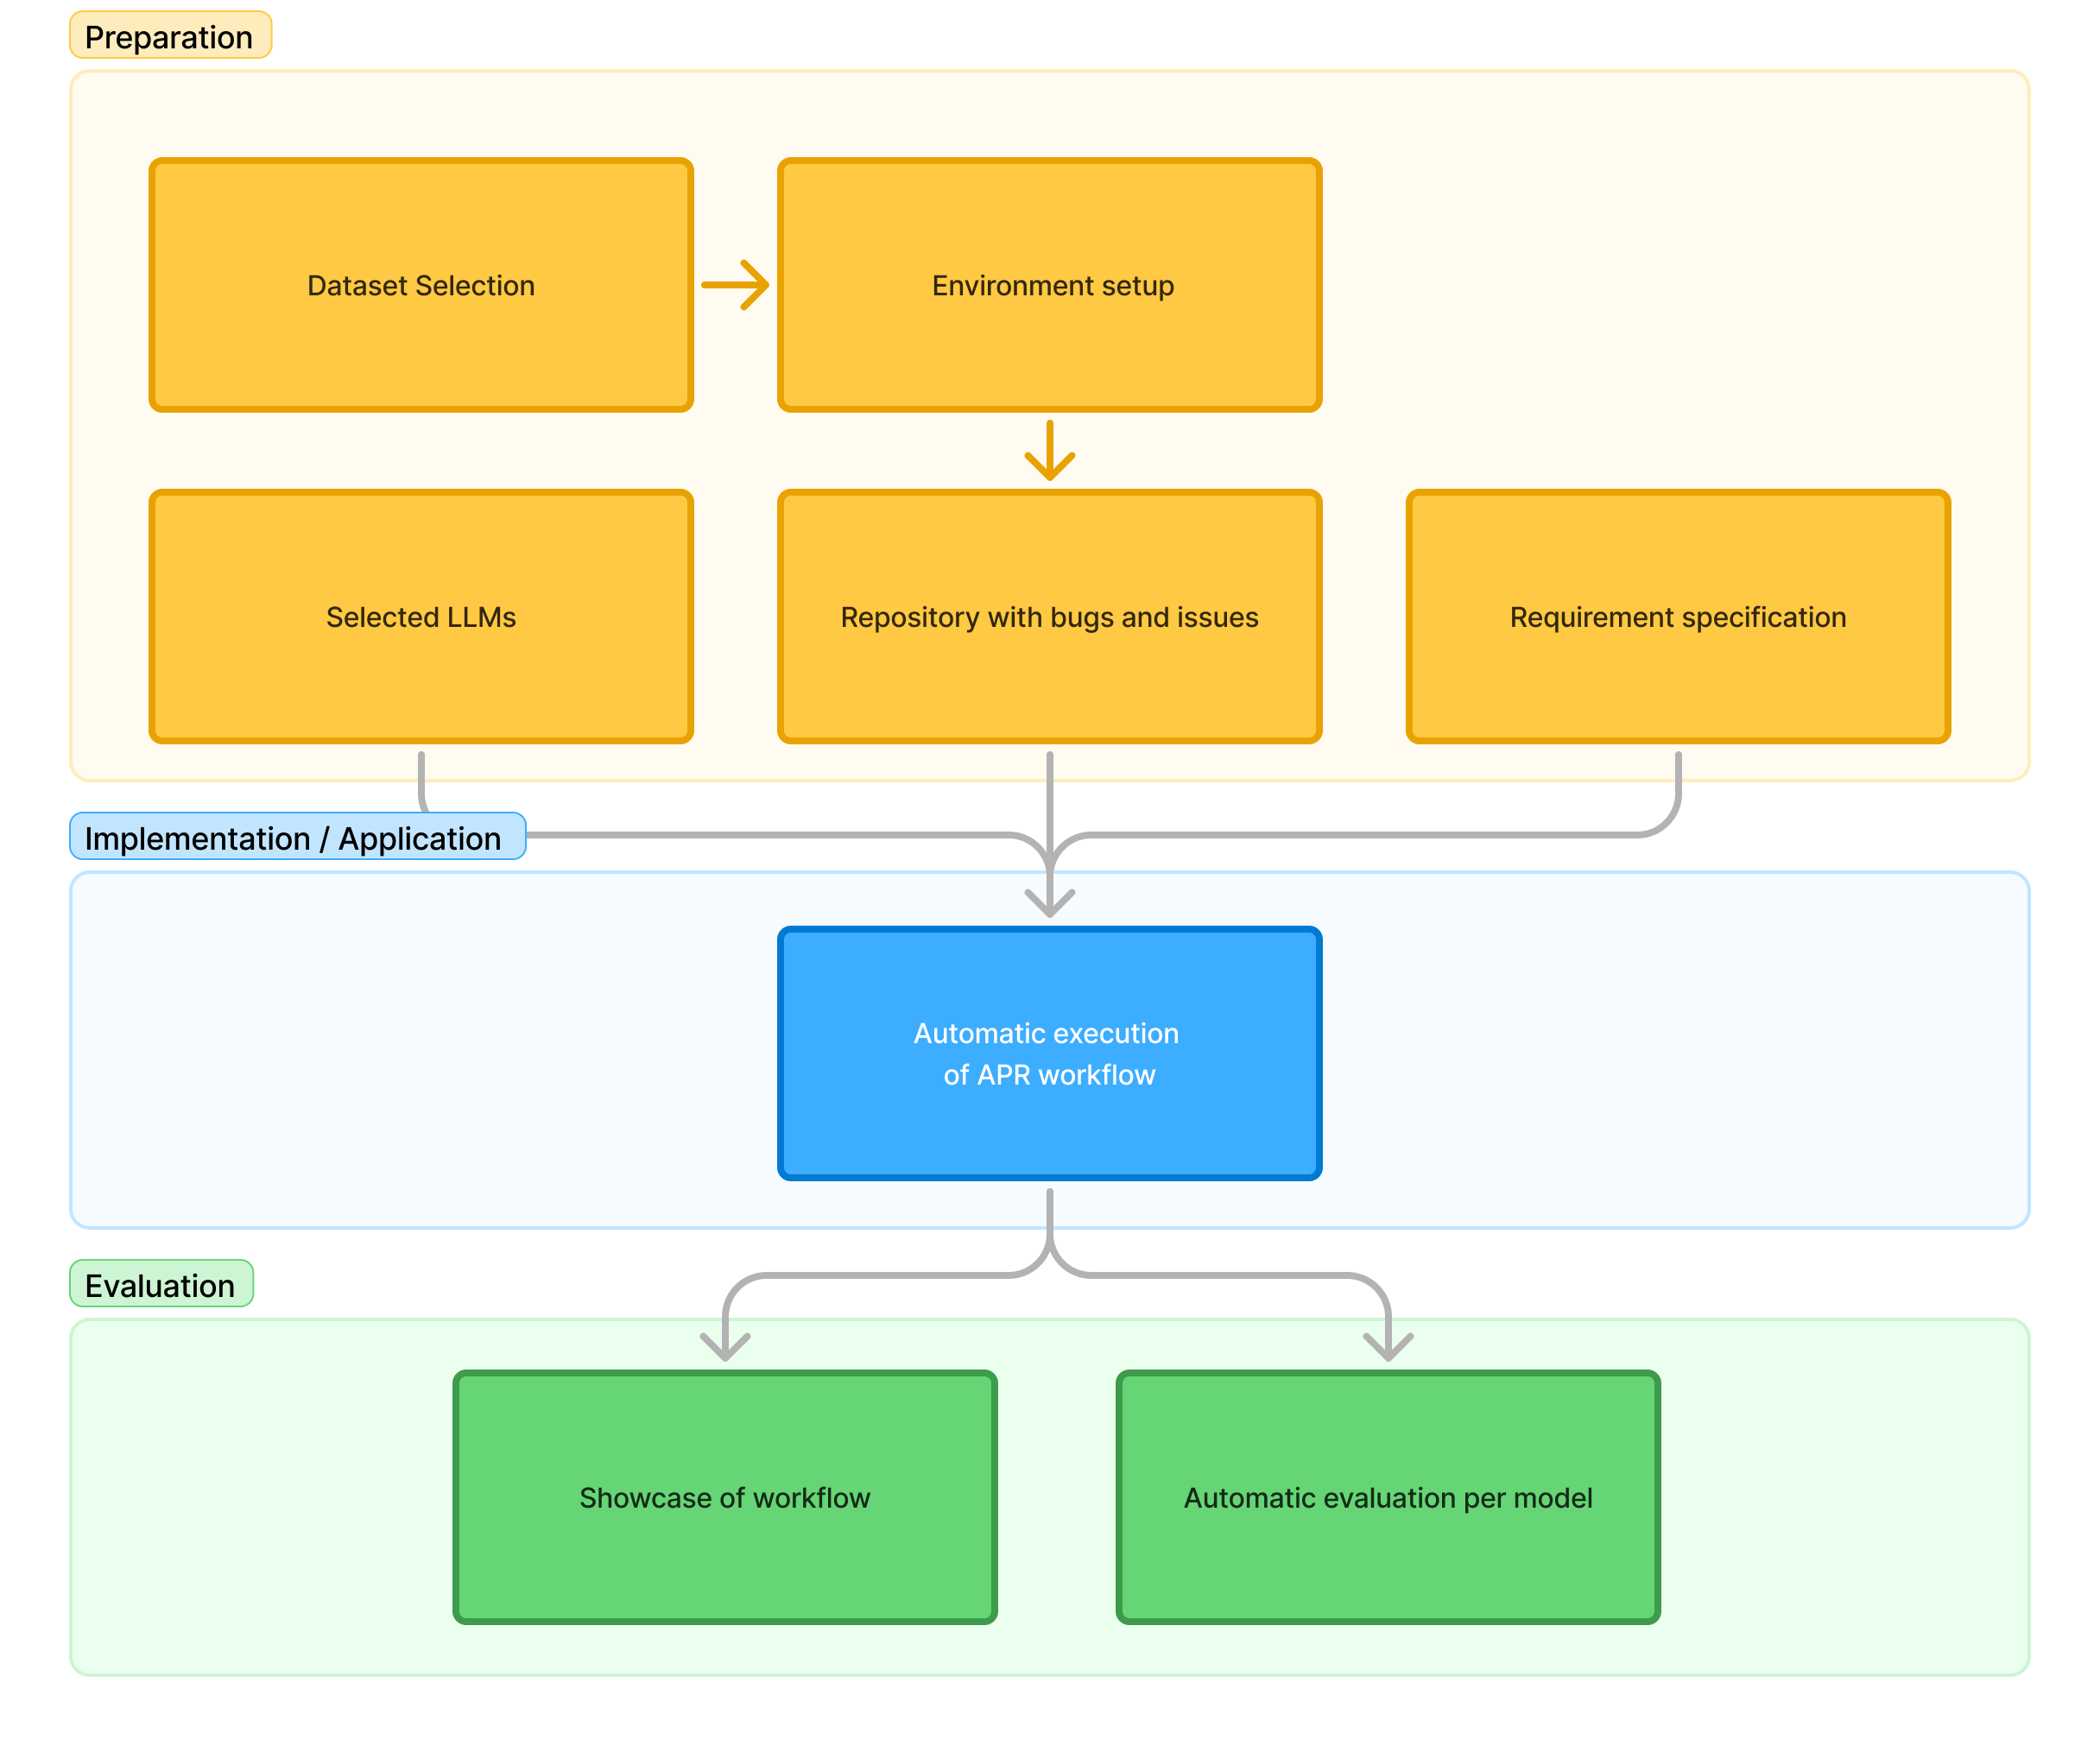
\includegraphics[width=0.8\textwidth]{images/flowcharts/method.png}
    \caption{Thesis Method Overview}
    \label{fig:method-overview}
\end{figure}

In the preparation we select a suitable APR benchmark. With this benchmark we set up a realistic development environment. By specifying requirements we lay the groundwork for the implementation of the APR system.
In the second part we implement the APR system as a GitHub Action workflow based on the requirements.
Lastly evaluation of the self developed prototype is done by using the defined evaluation metrics \ref{section:evaluation} collected during the execution of the APR system. Furthermore we will showcase the resulting workflow of using the system in a repository.
The following sections will go into detail of each of these phases.

\section{Preparation}
For implementing and evaluating our system we first need to prepare an environment where the system can be integrated and used. This includes selecting a suitable dataset, setting up the environment, and specifying the requirements for the system.
\subsection{Dataset Selection}
For the evaluation of our APR integration, we selected the QuixBugs benchmark \cite{linQuixBugsMultilingualProgram2017}. This dataset is well-suited for our purposes due to its focus on small-scale software bugs in Python. It consists of 40 individual files containing an algorithmic bug each. The bug is always caused by single erroneous line. QuixBugs brings corresponding tests and a corrected version for every file which allows for repair validation. The bugs where developed as challenging problems for developers \cite{linQuixBugsMultilingualProgram2017}, it enables us to evaluate if our system can take over the cognitive demanding task of fixing small bugs without developer intervention.

Compared to other APR benchmarks \ref{table:benchmarks} like SWE-Bench \cite{jimenezSWEbenchCanLanguage2024} QuixBugs is relatively small which allows for accelerated setup and development.

\subsection{LLM Selection} \label{subsection:llm-selection}
For the evaluation of our APR system we will test several LLM models. multiple smaller models for this benchmark to. these models are to have fast response times and low costs. For that we will compare a wide selection of recent (point 11.07.2025) models from different providers. The models are selected to cover a range of capabilities and costs in the lower tier, allowing us to evaluate the performance and cost-effectiveness of the APR system. The selected models are:
\begin{table}[ht]
    \centering
    \small
    \begin{tabular*}{\textwidth}{@{\extracolsep{\fill}} p{3cm} | p{2cm} | p{2cm} | p{4cm} | p{2cm}  @{}}
        \hline
        \textbf{Model Name} & \textbf{Publisher} & \textbf{Context Window Size} & \textbf{Cost per 1M} \\
        \hline
        \textbf{gemini-2.0-flash} & Google & 128k & input: \$0.10 output: \$0.40 \\
        \textbf{gemini-2.5-flash-lite} & Google & 128k & input: \$0.10 output: \$0.40 \\
        \textbf{gemini-2.5-flash} & Google & 128k & input: \$0.10 output: \$0.40 \\
        \textbf{gemini-2.5-pro} & Google & 128k & input: \$0.10 output: \$0.40 \\
        \textbf{gpt-4.1-nano} & OpenAI & 128k & input: \$0.10 output: \$0.40 \\
        \textbf{gpt-4.1-mini} & OpenAI & 128k & input: \$0.10 output: \$0.40 \\
        \textbf{gpt-4o} & OpenAI & 128k & input: \$0.10 output: \$0.40 \\
        \textbf{o4-mini} & OpenAI & 128k & input: \$0.10 output: \$0.40 \\
        \textbf{claude-3-haiku} & Anthropic & 128k & input: \$0.10 output: \$0.40 \\
        \textbf{claude-3-5-haiku} & Anthropic & 128k & input: \$0.10 output: \$0.40 \\
        \textbf{claude-3-7-sonnet} & Anthropic & 128k & input: \$0.10 output: \$0.40 \\
        \textbf{claude-sonnet-4-0} & Anthropic & 128k & input: \$0.10 output: \$0.40 \\
        \hline
    \end{tabular*}
    \caption{Selection of Large Language Models}
    \label{table:llms}
\end{table}

\subsection{Environment Setup} \label{subsection:environment-setup}
To mirror realistic software development environment, we prepared a GitHub repository containing the QuixBugs datasets python files. This repository serves as the basis for the bug fixing process, allowing the system to interact with the codebase and perform repairs. The repository contains only relevant files and folders required for the bug fixing process, ensuring a clean environment for the system to operate in.

Using the relevant files we generate a GitHub issue for each bug, using a consistent template that captures only the title of the Problem. These issues serve as the entry points and communication medium to our APR pipeline.

\begin{figure}[H]
    \centering
    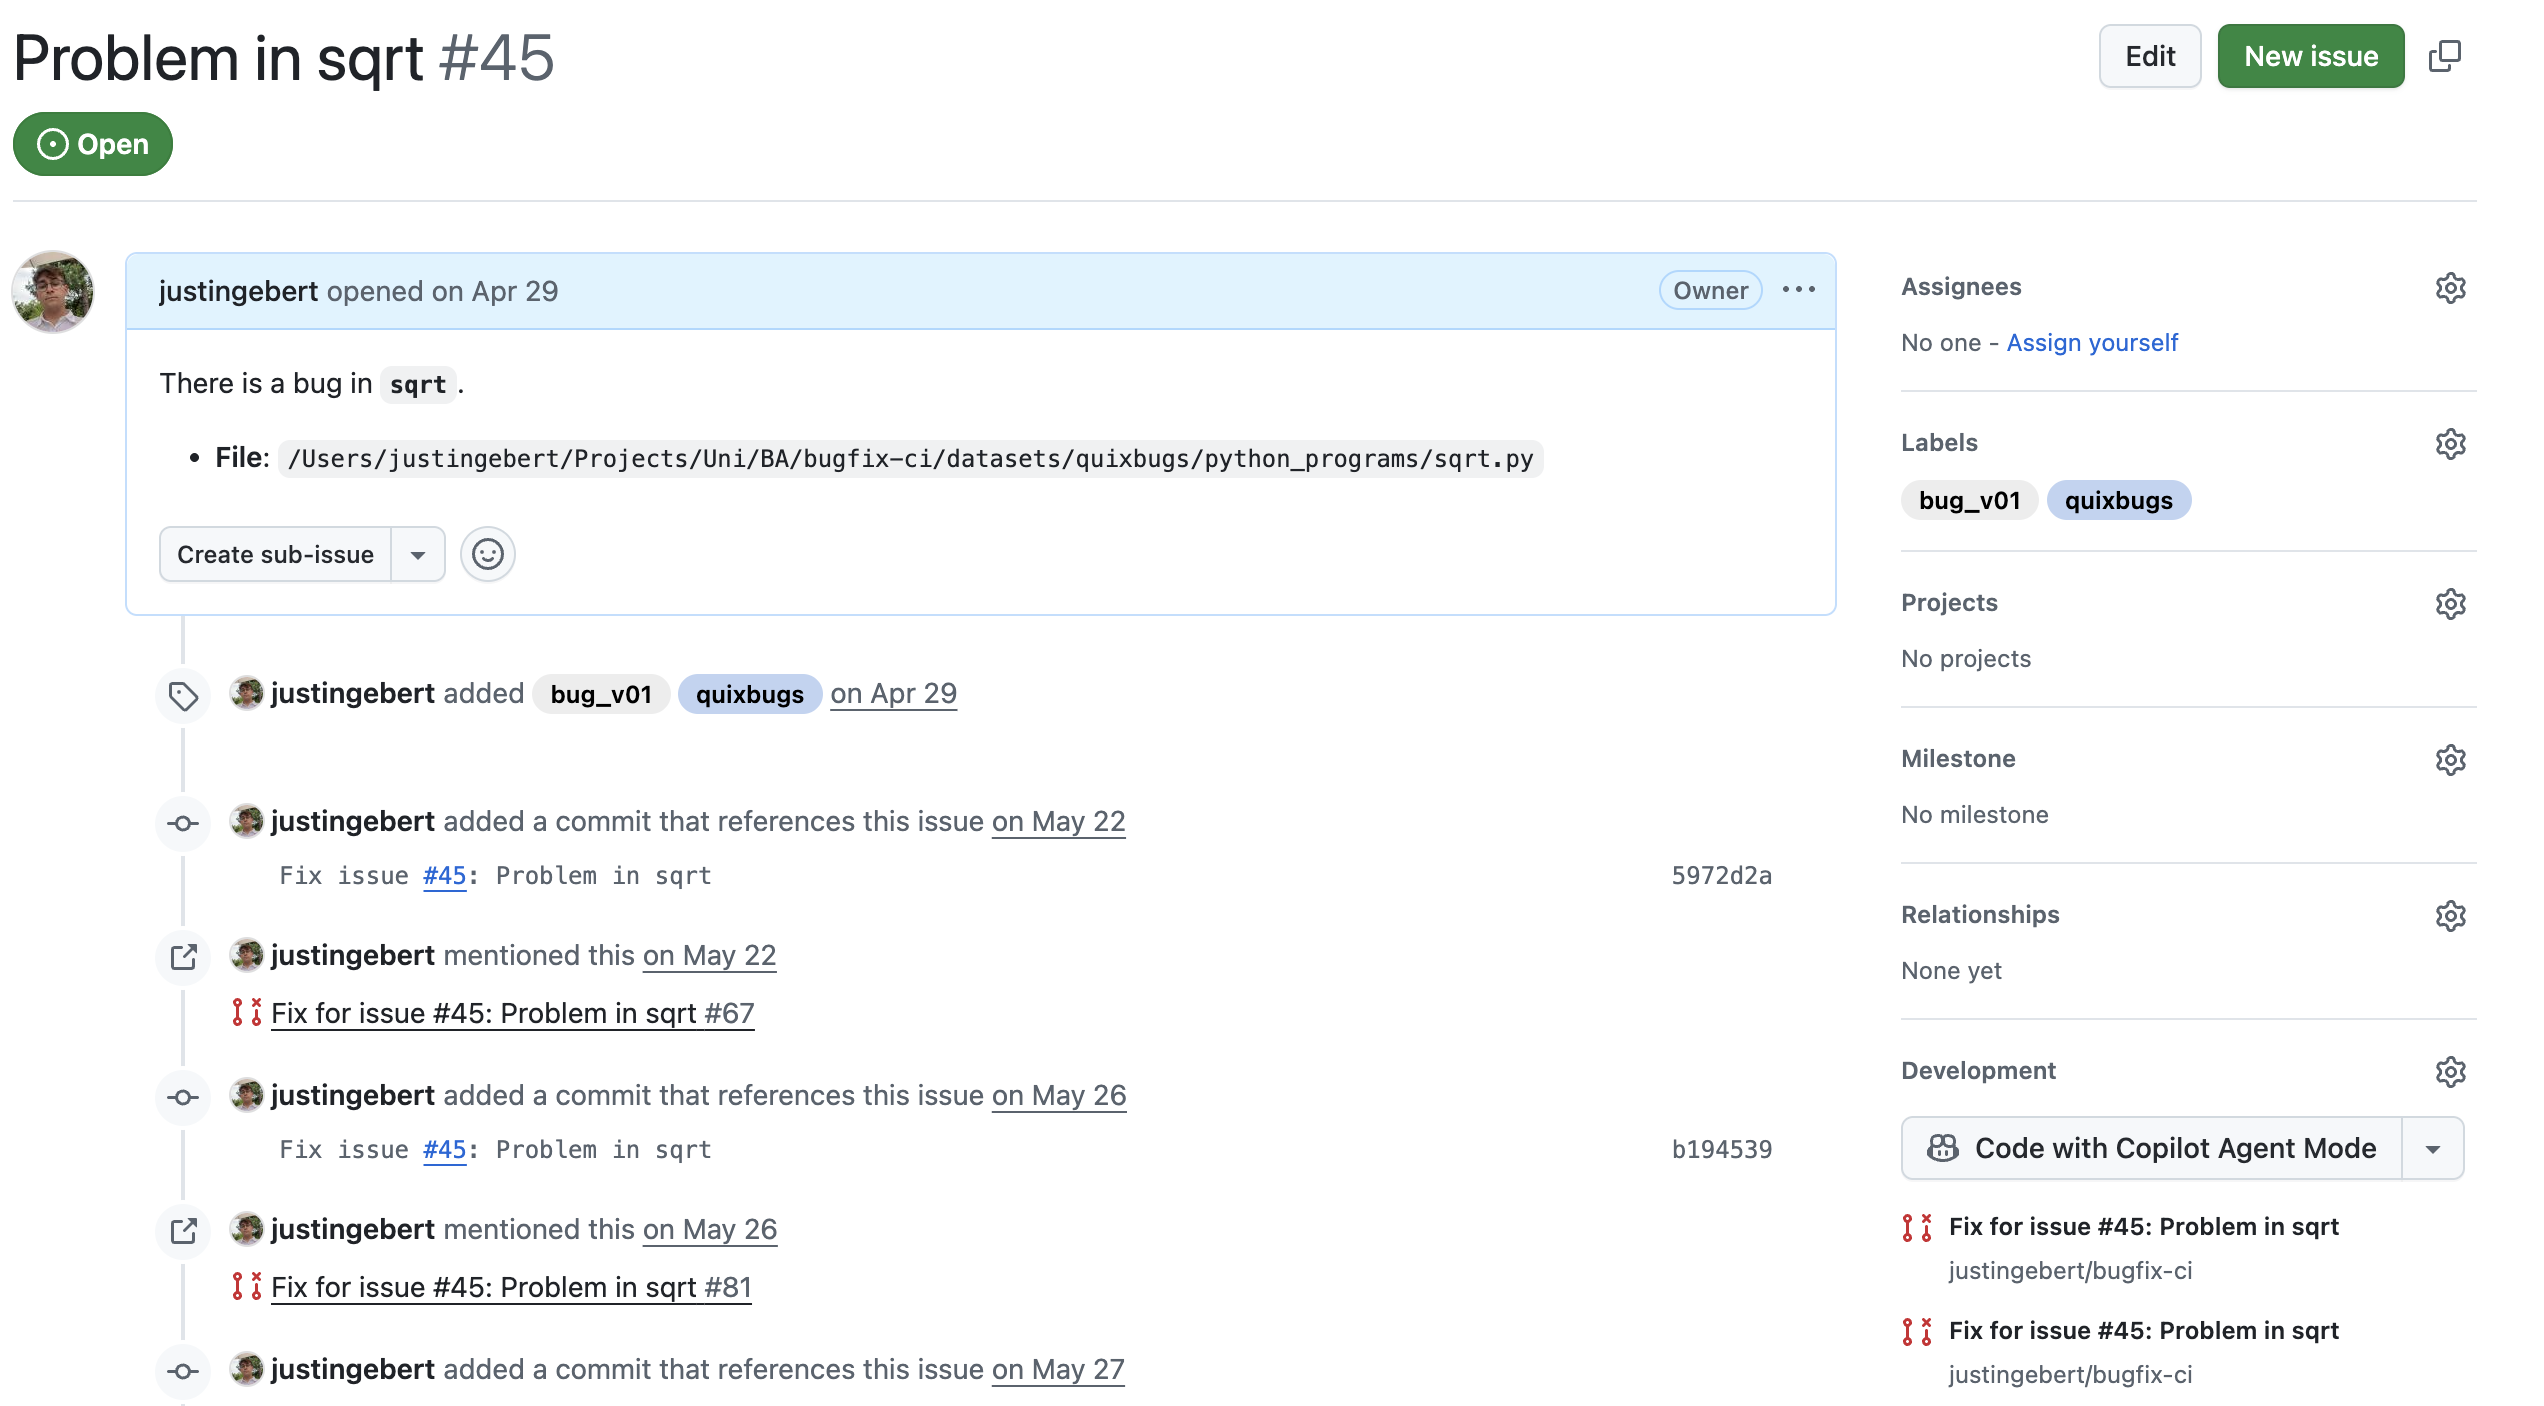
\includegraphics[width=1\textwidth]{images/github/GitHub Issue.png}
    \caption{Example of a GitHub Issue}
    \label{fig:gh-issue2}
\end{figure}

\subsection{Requirements Specification}

Before implementation we constructed the requirements for the prototype following the INVEST model, a widely-adopted method in Agile software development for engineering requirements \cite{10.5555/984017}. According to the INVEST principles, each requirement was formulated to be independent, negotiable, valuable, estimable, small, and testable. This model ensured that both functional and non-functional requirements were precisely defined, clearly verifiable, and easily adaptable to iterative development. The resulting requirements are detailed in \ref{chapter:requirements}.
\section{Pipeline Implementation}
In this section we will give a high-level overview of the implemented Automated Bug Fixing Pipeline. More detailed information about the implementation can be found in \ref{chapter:implementation}.

The Automated Bug Fixing Pipeline was developed using iterative prototyping and testing, with a focus on simplicity and extendability. Using the self developed requirements\ref{chapter:requirements} we build the following System:

\begin{figure}[H]
    \centering
    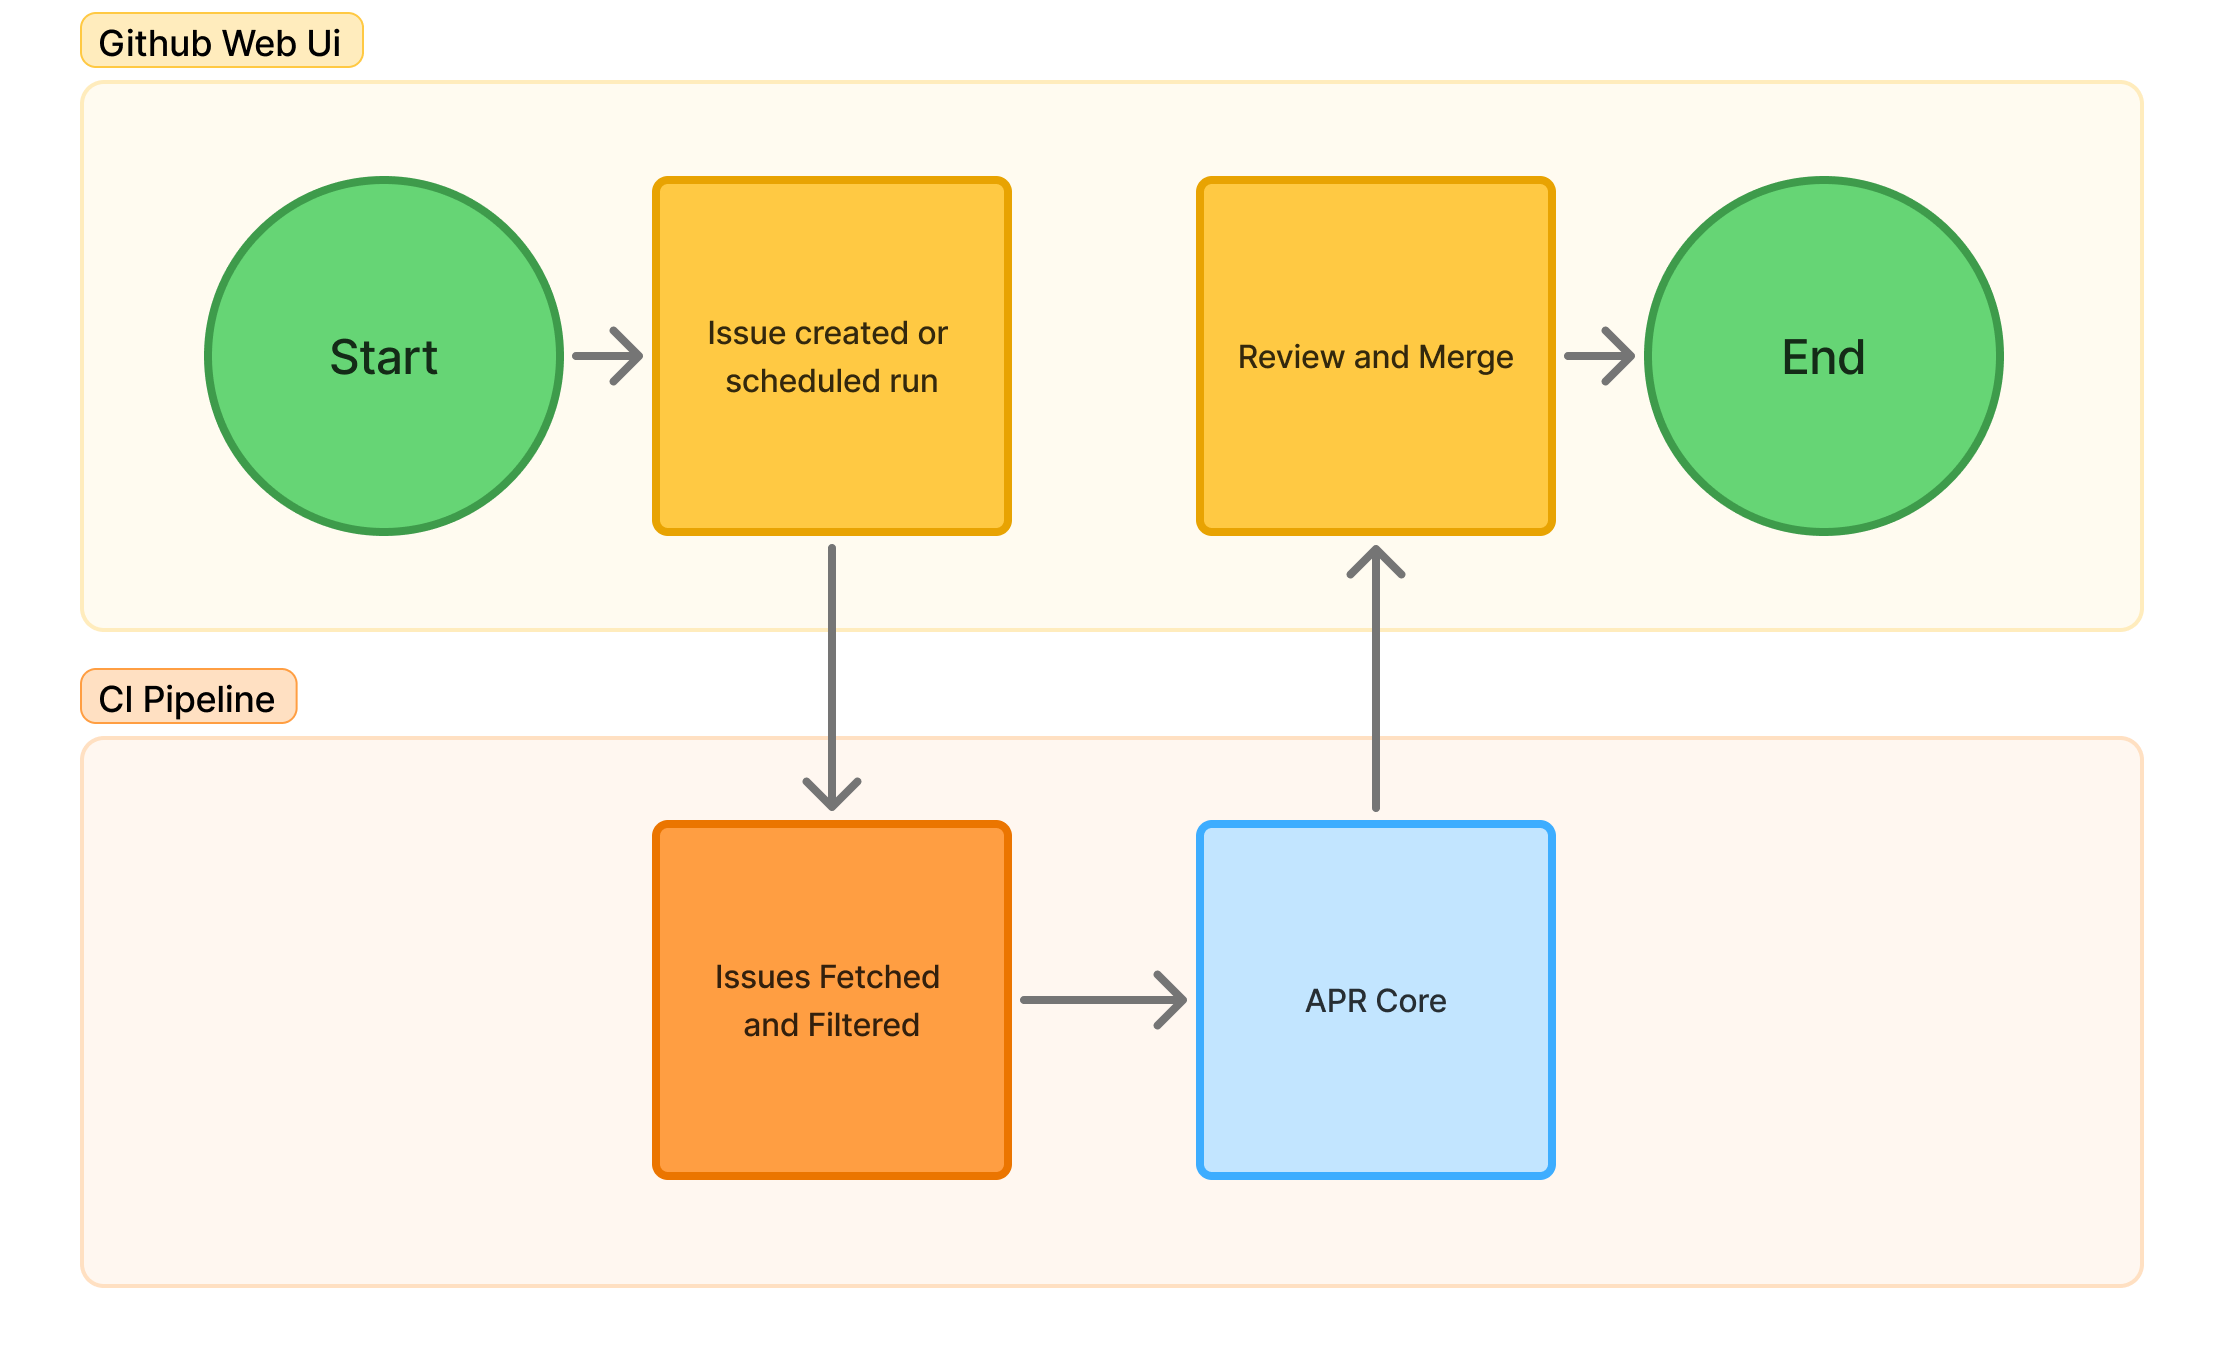
\includegraphics[width=1\textwidth]{images/flowcharts/high-level.png}
    \caption{High-Level Overview of the APR Pipeline}
    \label{fig:high-level}
\end{figure}

\begin{figure}[H]
    \centering
    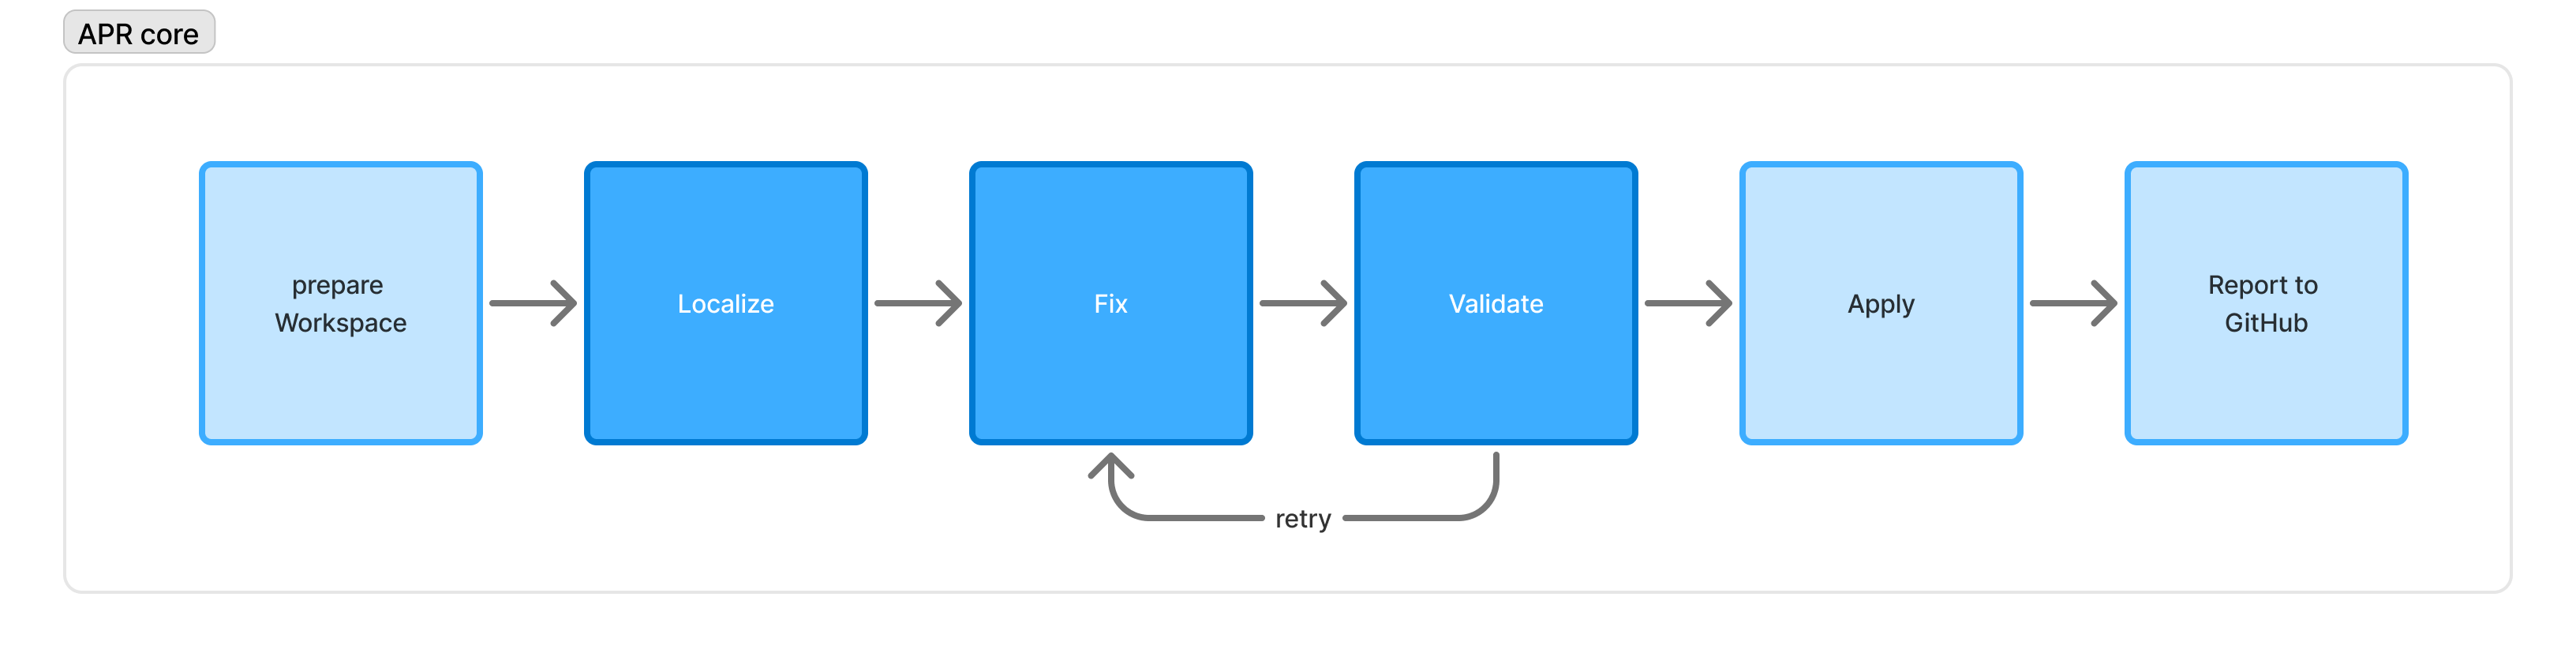
\includegraphics[width=1\textwidth]{images/flowcharts/agent-core-high-level.png}
    \caption{High-Level Overview of the APR Core}
    \label{fig:apr-core-high-level}
\end{figure}

When the system is in place in a target repository the pipeline can automatically be triggered by the configured triggers. On successful trigger a github action runner executes the pipeline. After entrypoint the relevant issues are selected and filtered for processing. The issues are the passed to the Dockerized APR system which talks to the configured LLM via API to localize and fix the issue. With the generated file edits the changes is validated and tested. When validation passes changes get applied and a pull request is automatically opened on the repository, linking the issue and providing details about the repair process. In case of a unsuccessful repair or exhaustion of the configured maximum attempts the failure is reported to the issue.

\section{Evaluation} \label{section:evaluation}

In this section, we describe how we measure the effectiveness, performance and cost of our APR pipeline when integrated into a Github repository. Using Github Actions Continuous Integration abilities, with our QuixBugs repository as a bases.  For this evaluation we selected a set of LLM models to be used for the APR process.

We focus on several key data metrics to assess the system's performance and abilities in repairing software bugs. These metrics will provide insights into the system's efficiency, reliability, and overall impact on the software development lifecycle.

For evaluating the effectiveness of the LLM model used and approach the determine the repair success rate. A success of an issue is determined by validation and the complete test suite provided by QuixBugs. An issues is considered successfully repaired when the validation passes with correct syntax and the test suite passes all tests.

Furthermore we will evaluate wether multiple attempts to repair an issue improve the repair success rate and how the number of attempts relates to the cost of repairing an issue.

For evaluating feasibility and performance evaluation we will analyze collected aggregated and fine grained timings and costs of a repair attempt.

The following data is automatically collected by each run of the APR pipeline. Using self developed scripts we collect the data from different sources for each run. Using this data to calculate the results defined in \ref{table:calculations}

\begin{table}[ht]
    \centering
    \small
    \renewcommand{\arraystretch}{1.5}
    \begin{tabular*}{\textwidth}{@{\extracolsep{\fill}} p{4cm} | p{6cm} | p{4cm} @{}}
        \toprule
        \textbf{Metric} & \textbf{Description} & \textbf{Source} \\
        \midrule
        Run ID & Unique identifier for each run of a Workflow & Github Action Env \\ \hline
        Model Used & LLM model used for the repair process & Configuration File \\ \hline
        Configuration & Configuration details, including LLM Model and settings & Target Github repository  \\ \hline
        Successful Repairs & Count of issues successfully repaired & APR Core \\ \hline
        Execution Time & Total time taken for the run & APR Core \\ \hline
        Job Execution Times & Time taken for each job in the pipeline & Github API \\ \hline
        Issues Processed & Information of Issues processed in the run \ref{table:issue-metrics} & APR Core \\
        \bottomrule
    \end{tabular*}
    \caption{Run Metrics Collected for each execution}
    \label{table:run-metrics}
\end{table}

Data collected for each issue processed by the APR core:

\begin{table}[H]
    \centering
    \small
    \renewcommand{\arraystretch}{1.5}
    \begin{tabular*}{\textwidth}{@{\extracolsep{\fill}} p{4cm} | p{6cm} | p{4cm} @{}}
        \toprule
        \textbf{Metric} & \textbf{Description} & \textbf{Source} \\
        \midrule
        Issue ID & Unique identifier of the issue processed & Github Issue ID \\ \hline
        Repair Successful & Boolean indicating whether the repair was successful. Tr & APR Core \\ \hline
        Number of Attempts & Total attempts made & APR Core \\ \hline
        Execution Time & Total time taken to process the issue, including all stages & APR Core \\ \hline
        Tokens Used & Number of tokens consumed by the LLM during the repair process & LLM API \\ \hline
        Cost & Cost associated with the repair process, calculated based on tokens and execution time & APR Core \\ \hline
        Stage Information & Details about each stage of the repair process, including execution time and outcome & APR Core \\
        \bottomrule
    \end{tabular*}
    \caption{Run Metrics Collected for each issue}
    \label{table:issue-metrics}
\end{table}

An attempt to repair an issue consists of multiple stages during the repair process, each with its own metrics. The following table summarizes the metrics collected for each stage:

\begin{table}[H]
    \centering
    \small
    \renewcommand{\arraystretch}{1.5}
    \begin{tabular*}{\textwidth}{@{\extracolsep{\fill}} p{4cm} | p{6cm} | p{4cm} @{}}
        \toprule
        \textbf{Metrics} & \textbf{Description} & \textbf{Source} \\
        \midrule
        Stage ID & Unique identifier for each stage in the repair process & APR Core \\ \hline
        Stage Execution Time & Time taken for each stage of the repair process & APR Core \\ \hline
        Stage Outcome & Outcome of each stage, indicating success, warning or failure & APR Core \\ \hline
        Stage Details & Additional details, such as error or warnings messages & APR Core \\
        \bottomrule
    \end{tabular*}
    \caption{Run Metrics Collected for each stage}
    \label{table:stage-metrics}
\end{table}

Using this data we calculate the following metrics for each LLM model:
%TODO add models

%TODO add calculations and check if all metrics are needed or evaluation

\begin{table}[H]
    \centering
    \small
    \renewcommand{\arraystretch}{1.5}
    \begin{tabular*}{\textwidth}{@{\extracolsep{\fill}} p{5cm} | p{10cm} @{}}
        \toprule
        \textbf{Metrics} &  \textbf{Calculation} \\
        \midrule
        Repair Success Rate & Number of Successful Repairs / Total Issues Processed \\ \hline
        Average Number of Attempts & Total Attempts / Total Issues Processed \\ \hline
        Average Execution Time & Total Execution Time / Total Issues Processed \\ \hline
        Average Tokens Used & Total Tokens Used / Total Issues Processed \\ \hline
        Average Cost & Total Cost / Total Issues Processed \\ \hline
        Average Stage Execution Time & Total Stage Execution Time / Total Stages Processed \\ \hline
        Average Stage Outcome Success Rate & Number of Successful Stages / Total Stages Processed \\
        \bottomrule
    \end{tabular*}
    \caption{Metrics Calculated from the collected data}
    \label{table:calculations}
\end{table}
